% !TEX root = slide_deck.tex
% ============================================================
%  slide_deck.tex  —  Tesi di Laurea Magistrale
%  Explainable AI in Sanità: Storytelling e Transformer per LOS
%  Candidato: Simone Garau  |  Relatore: Prof. Giorgio Leonardi
%  Anno Accademico 2024/2025
% ============================================================

\documentclass[aspectratio=169, 10pt]{beamer}

% ── Tema ────────────────────────────────────────────────────
\usetheme[progressbar=frametitle, block=fill]{metropolis}

% ── Pacchetti ───────────────────────────────────────────────
\usepackage[italian]{babel}
\usepackage[utf8]{inputenc}
\usepackage[T1]{fontenc}
\usepackage{graphicx}
\usepackage{booktabs}
\usepackage{amsmath}
\usepackage{amssymb}
\usepackage{mathtools}       % \Coloneqq
\usepackage{multirow}
\usepackage{tikz}
\usetikzlibrary{positioning, arrows.meta}
\usepackage{xcolor}
\usepackage{fontawesome5}    % icone opzionali
\usepackage{hyperref}
\usepackage{appendixnumberbeamer} % numerazione separata slide backup

% Path immagini relativo alla cartella presentation/
\graphicspath{{../img/}}

% ── Palette Colori ───────────────────────────────────────────
% Blu navy accademico + arancio caldo
\definecolor{primary}{HTML}{1B3A6B}
\definecolor{accent}{HTML}{E07B39}
\definecolor{lightbg}{HTML}{F2F5FA}
\definecolor{darktext}{HTML}{2C2C2C}
\definecolor{alertred}{HTML}{C0392B}
\definecolor{successgreen}{HTML}{1A7A4A}

% ── Configurazione Metropolis ────────────────────────────────
\setbeamercolor{normal text}{fg=darktext, bg=lightbg}
\setbeamercolor{frametitle}{bg=primary, fg=white}
\setbeamercolor{progress bar}{fg=accent, bg=primary!30}
\setbeamercolor{title separator}{fg=accent}
\setbeamercolor{palette primary}{bg=primary}
\setbeamercolor{alerted text}{fg=accent}
\setbeamercolor{block title}{bg=primary!15, fg=primary}
\setbeamercolor{block body}{bg=primary!5, fg=darktext}
\setbeamercolor{block title alerted}{bg=alertred!20, fg=alertred!90!black}
\setbeamercolor{block body alerted}{bg=alertred!5, fg=darktext}
\setbeamercolor{block title example}{bg=successgreen!15, fg=successgreen!80!black}
\setbeamercolor{block body example}{bg=successgreen!5, fg=darktext}
\setbeamercolor{itemize item}{fg=accent}
\setbeamercolor{itemize subitem}{fg=primary}
\setbeamercolor{section in toc}{fg=primary}

\setbeamerfont{title}{size=\large, series=\bfseries}
\setbeamerfont{subtitle}{size=\normalsize, series=\mdseries}
\setbeamerfont{frametitle}{size=\normalsize, series=\bfseries}
\setbeamerfont{block title}{series=\bfseries}

% Footer personalizzato:
\setbeamertemplate{footline}{%
  \leavevmode%
  \begin{beamercolorbox}[wd=\paperwidth, leftskip=0.3cm, rightskip=0.3cm, dp=1.5ex, ht=2.5ex]{page number in head/foot}%
    \usebeamerfont{page number in head/foot}%
    {\tiny \insertshorttitle}%
    \hfill%
    {\tiny \insertframenumber\,/\,\inserttotalframenumber}%
  \end{beamercolorbox}%
  \vspace*{0.1cm} % Un piccolo margine inferiore per non tagliare le lettere (dp)
}
\setbeamercolor{page number in head/foot}{fg=darktext!55, bg=lightbg}

% ── Metadati ─────────────────────────────────────────────────
\title{Explainable AI in Sanità}
\subtitle{Storytelling e Modelli Transformer\\per l'Ottimizzazione del Length of Stay}
\author{Simone Garau}
\institute{%
  Università degli Studi del Piemonte Orientale\\
  Dipartimento di Scienze e Innovazione Tecnologica\\
  \smallskip
  {\small Relatore: Prof.\ Giorgio Leonardi}
}
\date{Anno Accademico 2024/2025}

% ============================================================
\begin{document}
% ============================================================

% ── SLIDE 1: Frontespizio ────────────────────────────────────
{
  \setbeamertemplate{footline}{}  % niente footer sul titolo
  \begin{frame}[noframenumbering]
    \begin{columns}[c]
      \begin{column}{0.22\textwidth}
        \centering
        
\includegraphics[width=\linewidth]{logo_upo.jpg}
      \end{column}
      \begin{column}{0.76\textwidth}
        \titlepage
      \end{column}
    \end{columns}
  \end{frame}
}

% ── SLIDE 2: Il Problema — LOS ───────────────────────────────
\section{Contesto e Motivazione}

\begin{frame}{Il Problema: Length of Stay (LOS)}
  \begin{columns}[T]
    \begin{column}{0.52\textwidth}
      \textbf{Cos'è il LOS?}\\
      La \alert{durata della degenza ospedaliera} è un indicatore
      critico di efficienza clinica e sostenibilità economica.

      \vspace{0.4em}
      \begin{block}{Soglia Critica}
        Degenze $\ge 20$ giorni classificate come \textbf{long-LOS}:\\
        sovraccarico di letti, rischio nosocomiale, costi elevati.
      \end{block}

      \vspace{0.4em}
      \textbf{Il dataset:}
      \begin{itemize}
        \item 7.393 casi clinici unici
        \item 88.115 eventi granulari
        \item Solo \alert{809 ($\approx$11\%)} con LOS critico
        \item Ospedale di Alessandria — 20 DRG
      \end{itemize}
    \end{column}

    \begin{column}{0.45\textwidth}
      \centering
      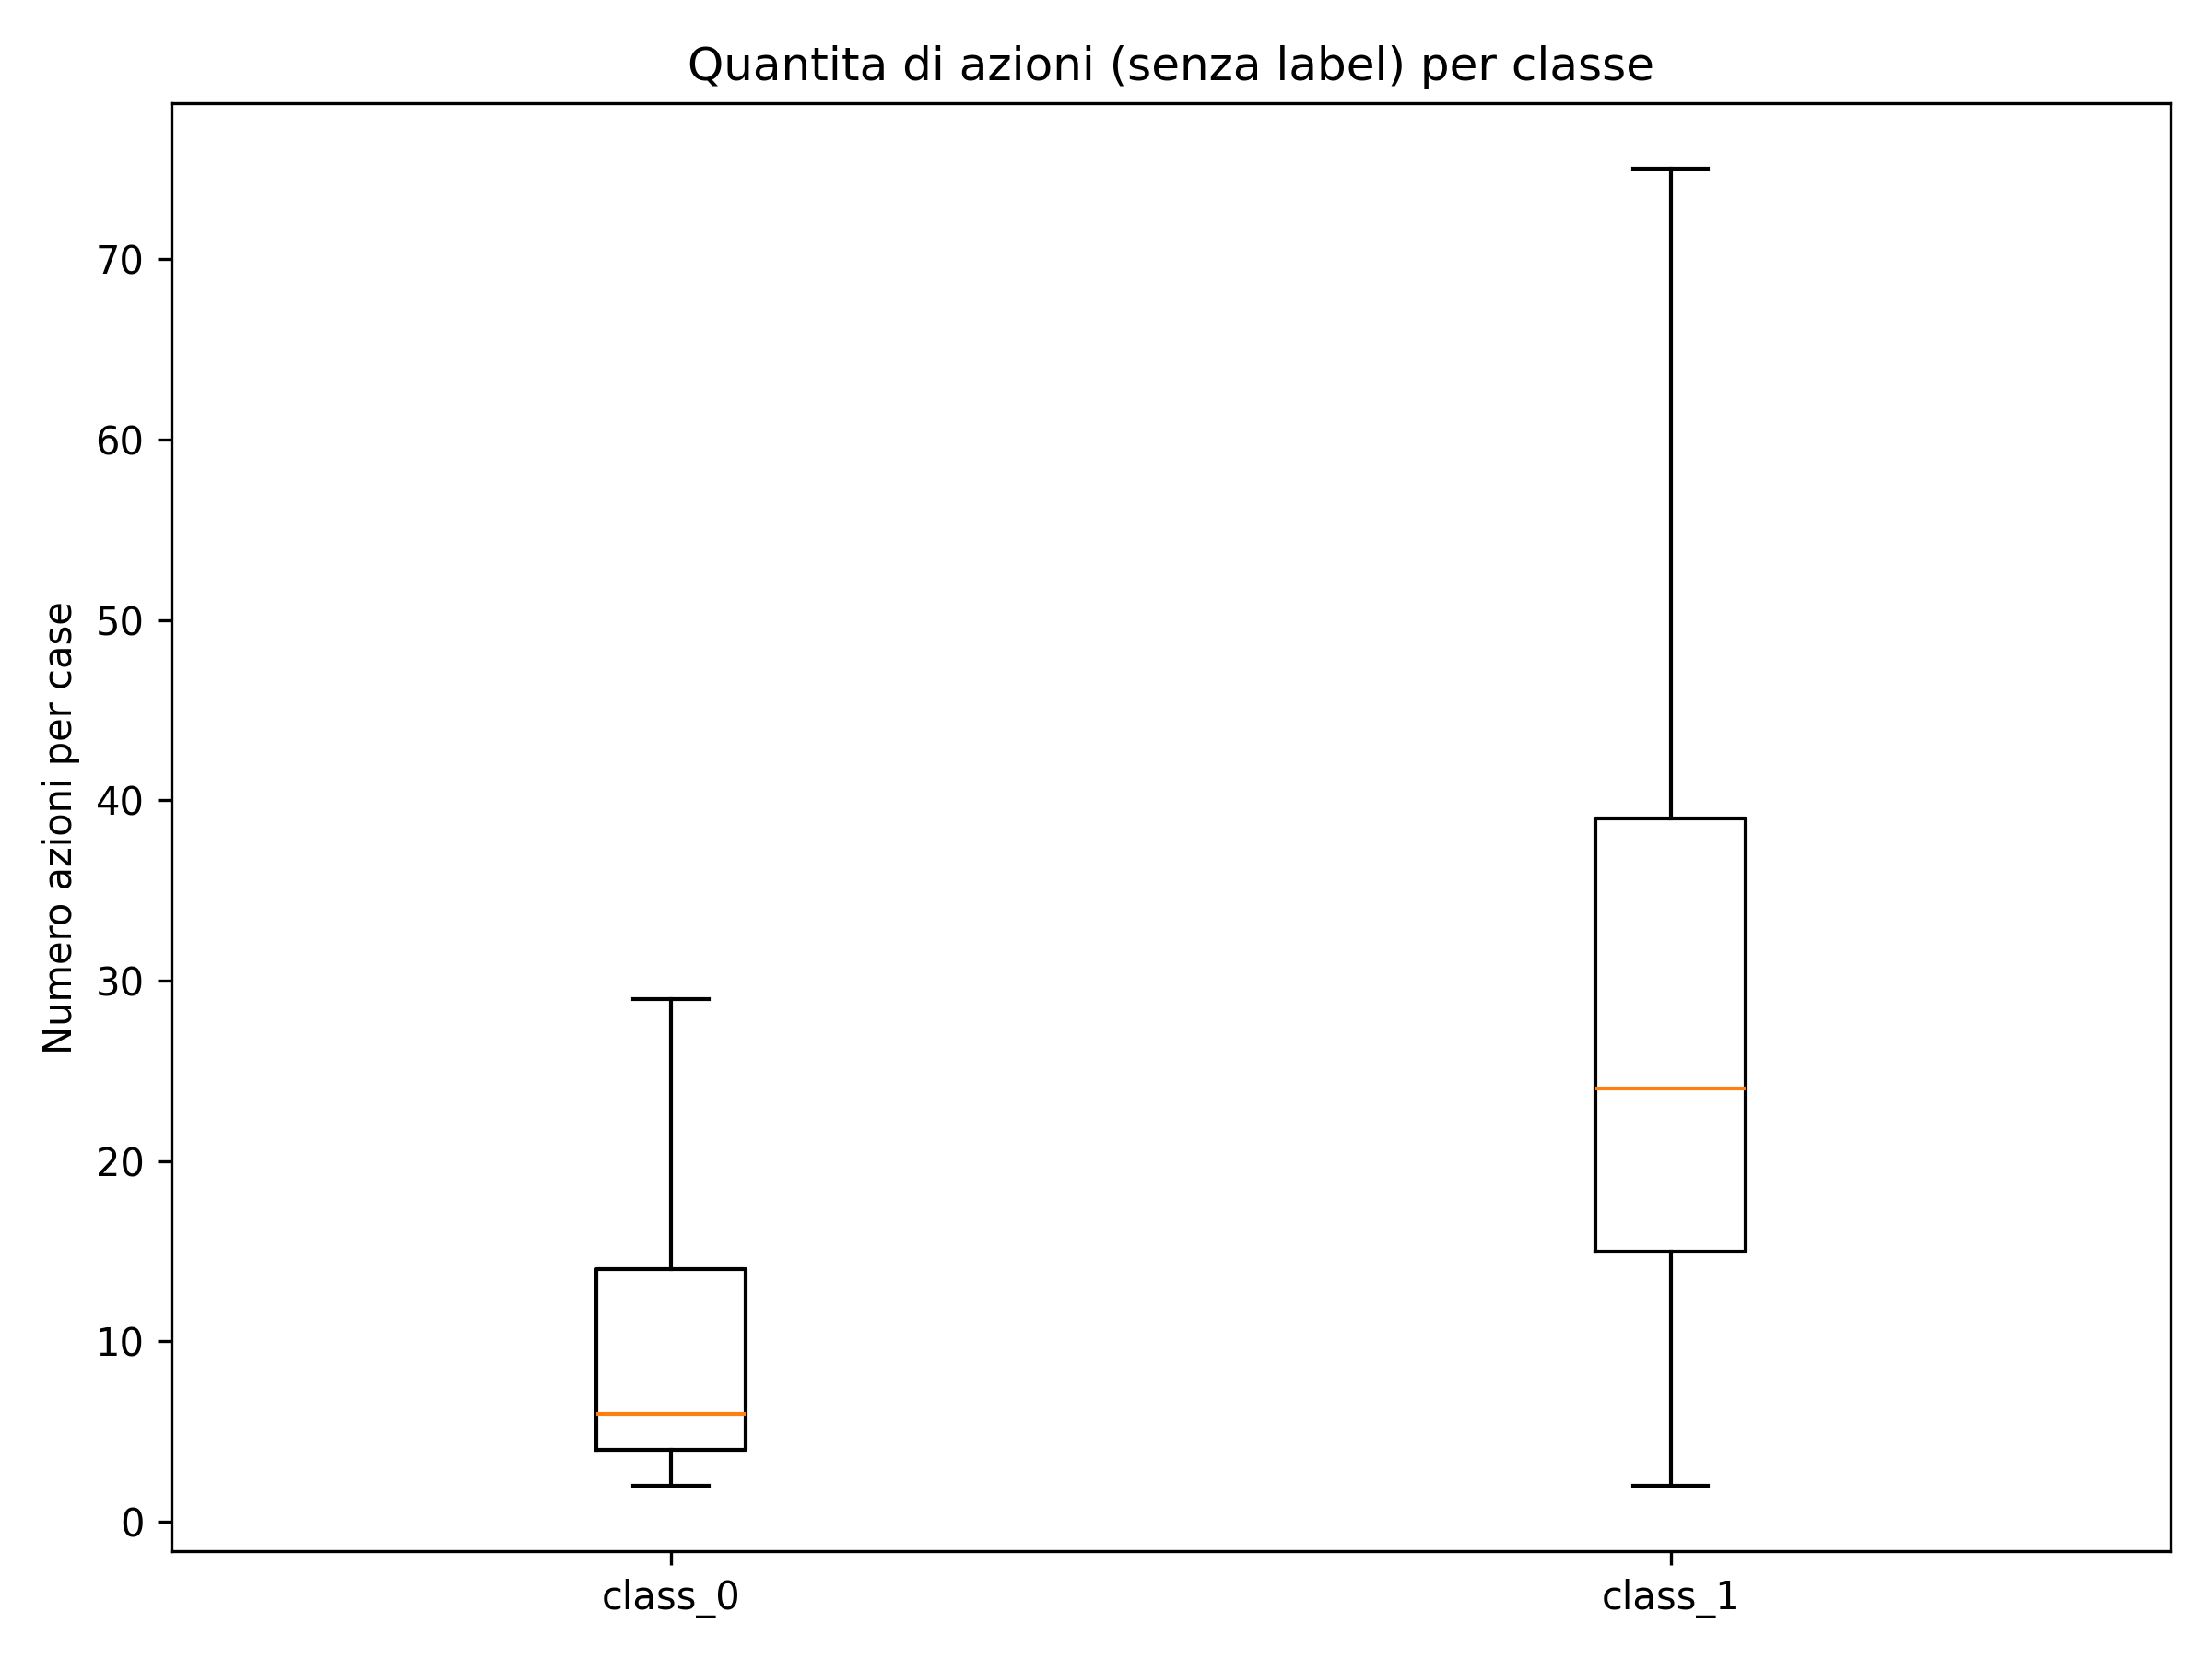
\includegraphics[width=\linewidth]{class_quantity_boxplot.png}
      {\small\itshape Numero d'azioni per classe:\\ i casi critici hanno percorsi molto più lunghi.}
    \end{column}
  \end{columns}
\end{frame}

% ── SLIDE 3: Limiti Process Mining ───────────────────────────
\begin{frame}{I Limiti dell'Approccio Classico}
  \begin{columns}[T]
    \begin{column}{0.55\textwidth}
      \textbf{Process Mining tradizionale:}
      \begin{itemize}
        \item Estrae grafi deterministici da log XES
        \item Modella flussi di cura e deviazioni standard
        \item Efficace per processi stabili e a bassa variabilità
      \end{itemize}

      \vspace{0.5em}
      \begin{alertblock}{Le Criticità sui Log Clinici}
        \begin{itemize}
          \item Alta variabilità e rumore nei log reali
          \item Dipendenze temporali a lungo termine
          \item Complessità semantica delle azioni cliniche
        \end{itemize}
      \end{alertblock}

      \vspace{0.4em}
      \textbf{Serve un modello capace di comprendere\\
      il \alert{contesto bidirezionale} di una sequenza.}
    \end{column}

    \begin{column}{0.42\textwidth}
      \centering
      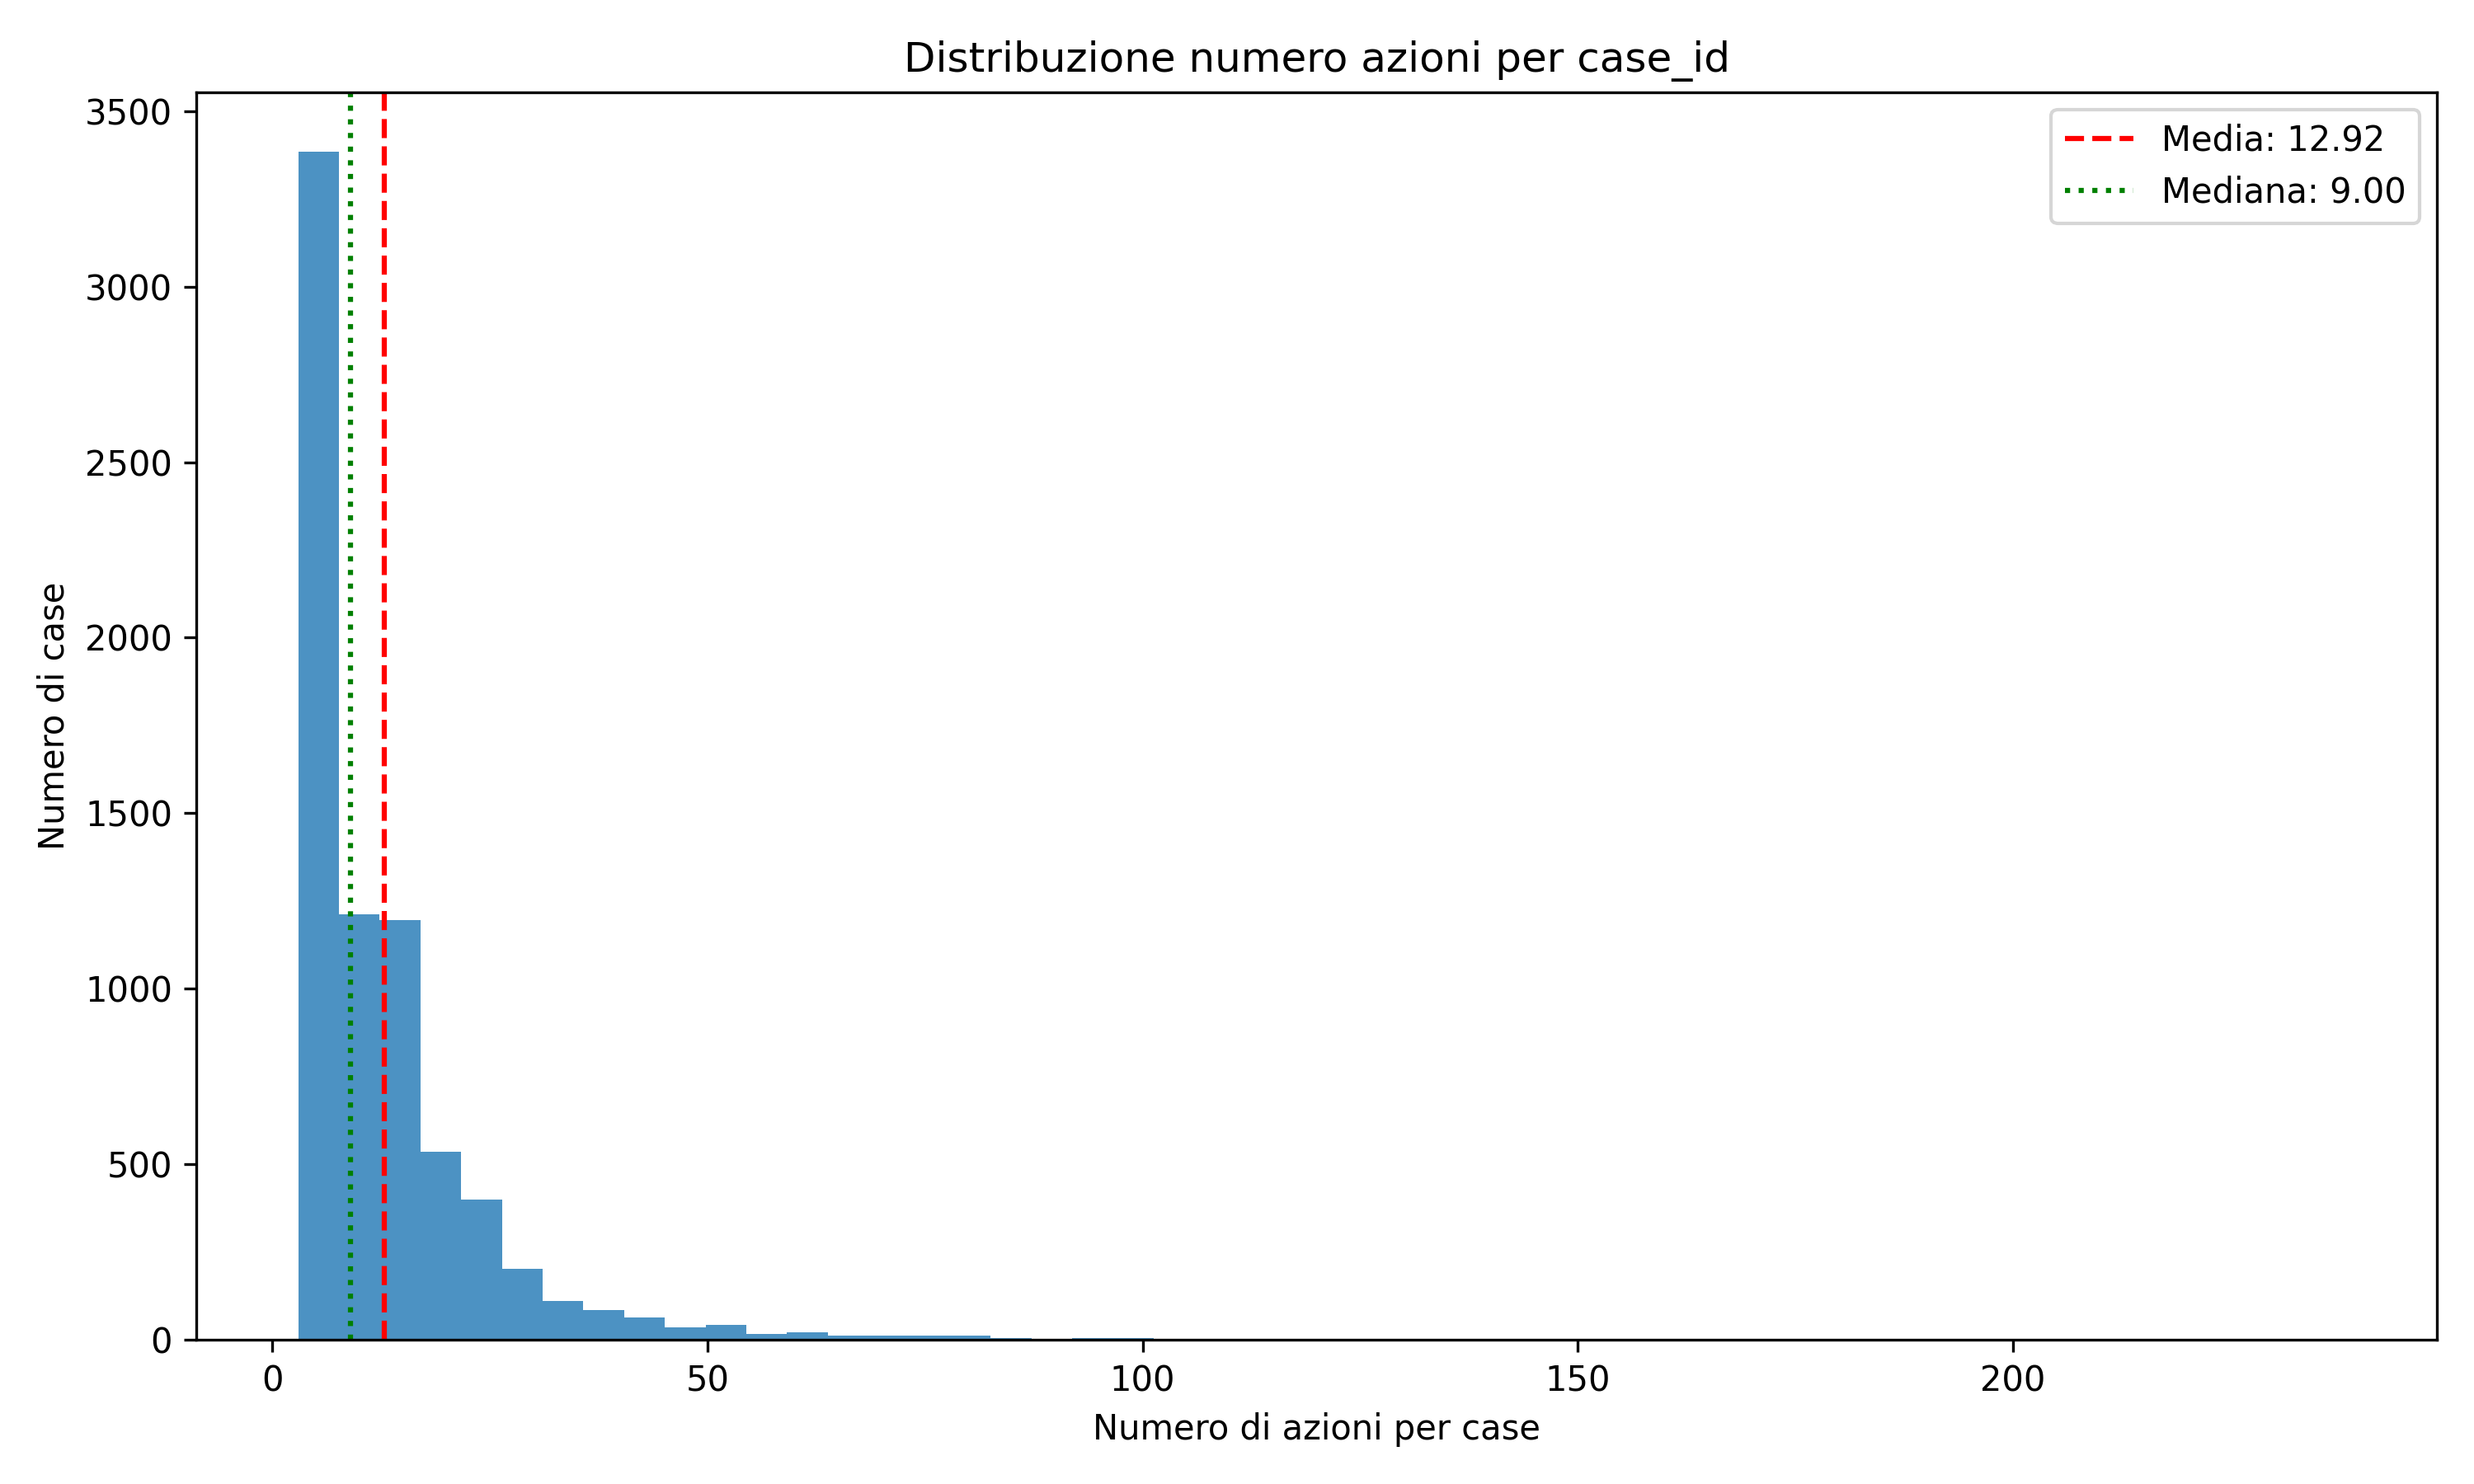
\includegraphics[width=\linewidth]{actions_per_case_distribution.png}
      {\small\itshape Distribuzione azioni per paziente:\\
      coda lunga $\to$ alta variabilità da gestire.}
    \end{column}
  \end{columns}
\end{frame}

% ── SLIDE 4: Storytelling ─────────────────────────────────────
\section{Metodologia}

\begin{frame}{L'Intuizione: il Paradigma ``Storytelling''}
  \textbf{Idea fondamentale:} tradurre una traccia clinica in un\\\textbf{testo narrativo in lingua naturale} processabile da BERT.

  \vspace{0.5em}
  \begin{columns}[T]
    \begin{column}{0.48\textwidth}
      \begin{block}{Da Log XES\ldots}
        \texttt{case\_id: 5870415}\\
        \texttt{--> Complete abdomen ultrasound}\\
        \texttt{--> CT skull} \quad$\Delta = 0$~s\\
        \texttt{--> Complete abdomen ultrasound} \quad$\Delta = 728.160$~s
      \end{block}
    \end{column}
    \begin{column}{0.48\textwidth}
      \begin{exampleblock}{\ldots a Narrazione}
        \small
        \textit{``The patient, 87 years old, underwent a series of
        examinations. After 0 seconds, the following examinations
        were performed simultaneously: Complete abdomen ultrasound
        and CT skull. After 728,160 seconds, Complete abdomen
        ultrasound was performed.''}
      \end{exampleblock}
    \end{column}
  \end{columns}

  \vspace{0.5em}
  \begin{alertblock}{Perché Storytelling vince sulle alternative?}
    Testati 3 embedding (binning temporale, array concatenati, storytelling).\\
    Lo storytelling porta la \textbf{Balanced Accuracy a 89.69\%},
    massimizzando il contesto semantico per BERT.
  \end{alertblock}
\end{frame}

% ── SLIDE 5: Dataset e Sbilanciamento ────────────────────────
\begin{frame}{Dataset e la Sfida dello Sbilanciamento}
  \begin{columns}[T]
    \begin{column}{0.50\textwidth}
      \begin{block}{EDA — Analisi Esplorativa}
        \begin{itemize}
          \item \textbf{7.393} casi | \textbf{88.115} eventi
          \item Media: \textbf{12.92} azioni/paziente
          \item Mediana: 9.00 azioni $\to$ distribuzione \textit{right-skewed}
        \end{itemize}
      \end{block}

      \vspace{0.4em}
      \textbf{Sbilanciamento di Classe:}
      \begin{itemize}
        \item Classe 0 (normale): \textbf{6.584} casi — 89\%
        \item Classe 1 (LOS $\ge 20$ gg): \alert{\textbf{809}} casi — 11\%
      \end{itemize}

      \vspace{0.4em}
      Una BCE standard collassa sulla classe maggioritaria.\\
      \textbf{Soluzione: Focal Loss.}
    \end{column}

    \begin{column}{0.47\textwidth}
      \centering
      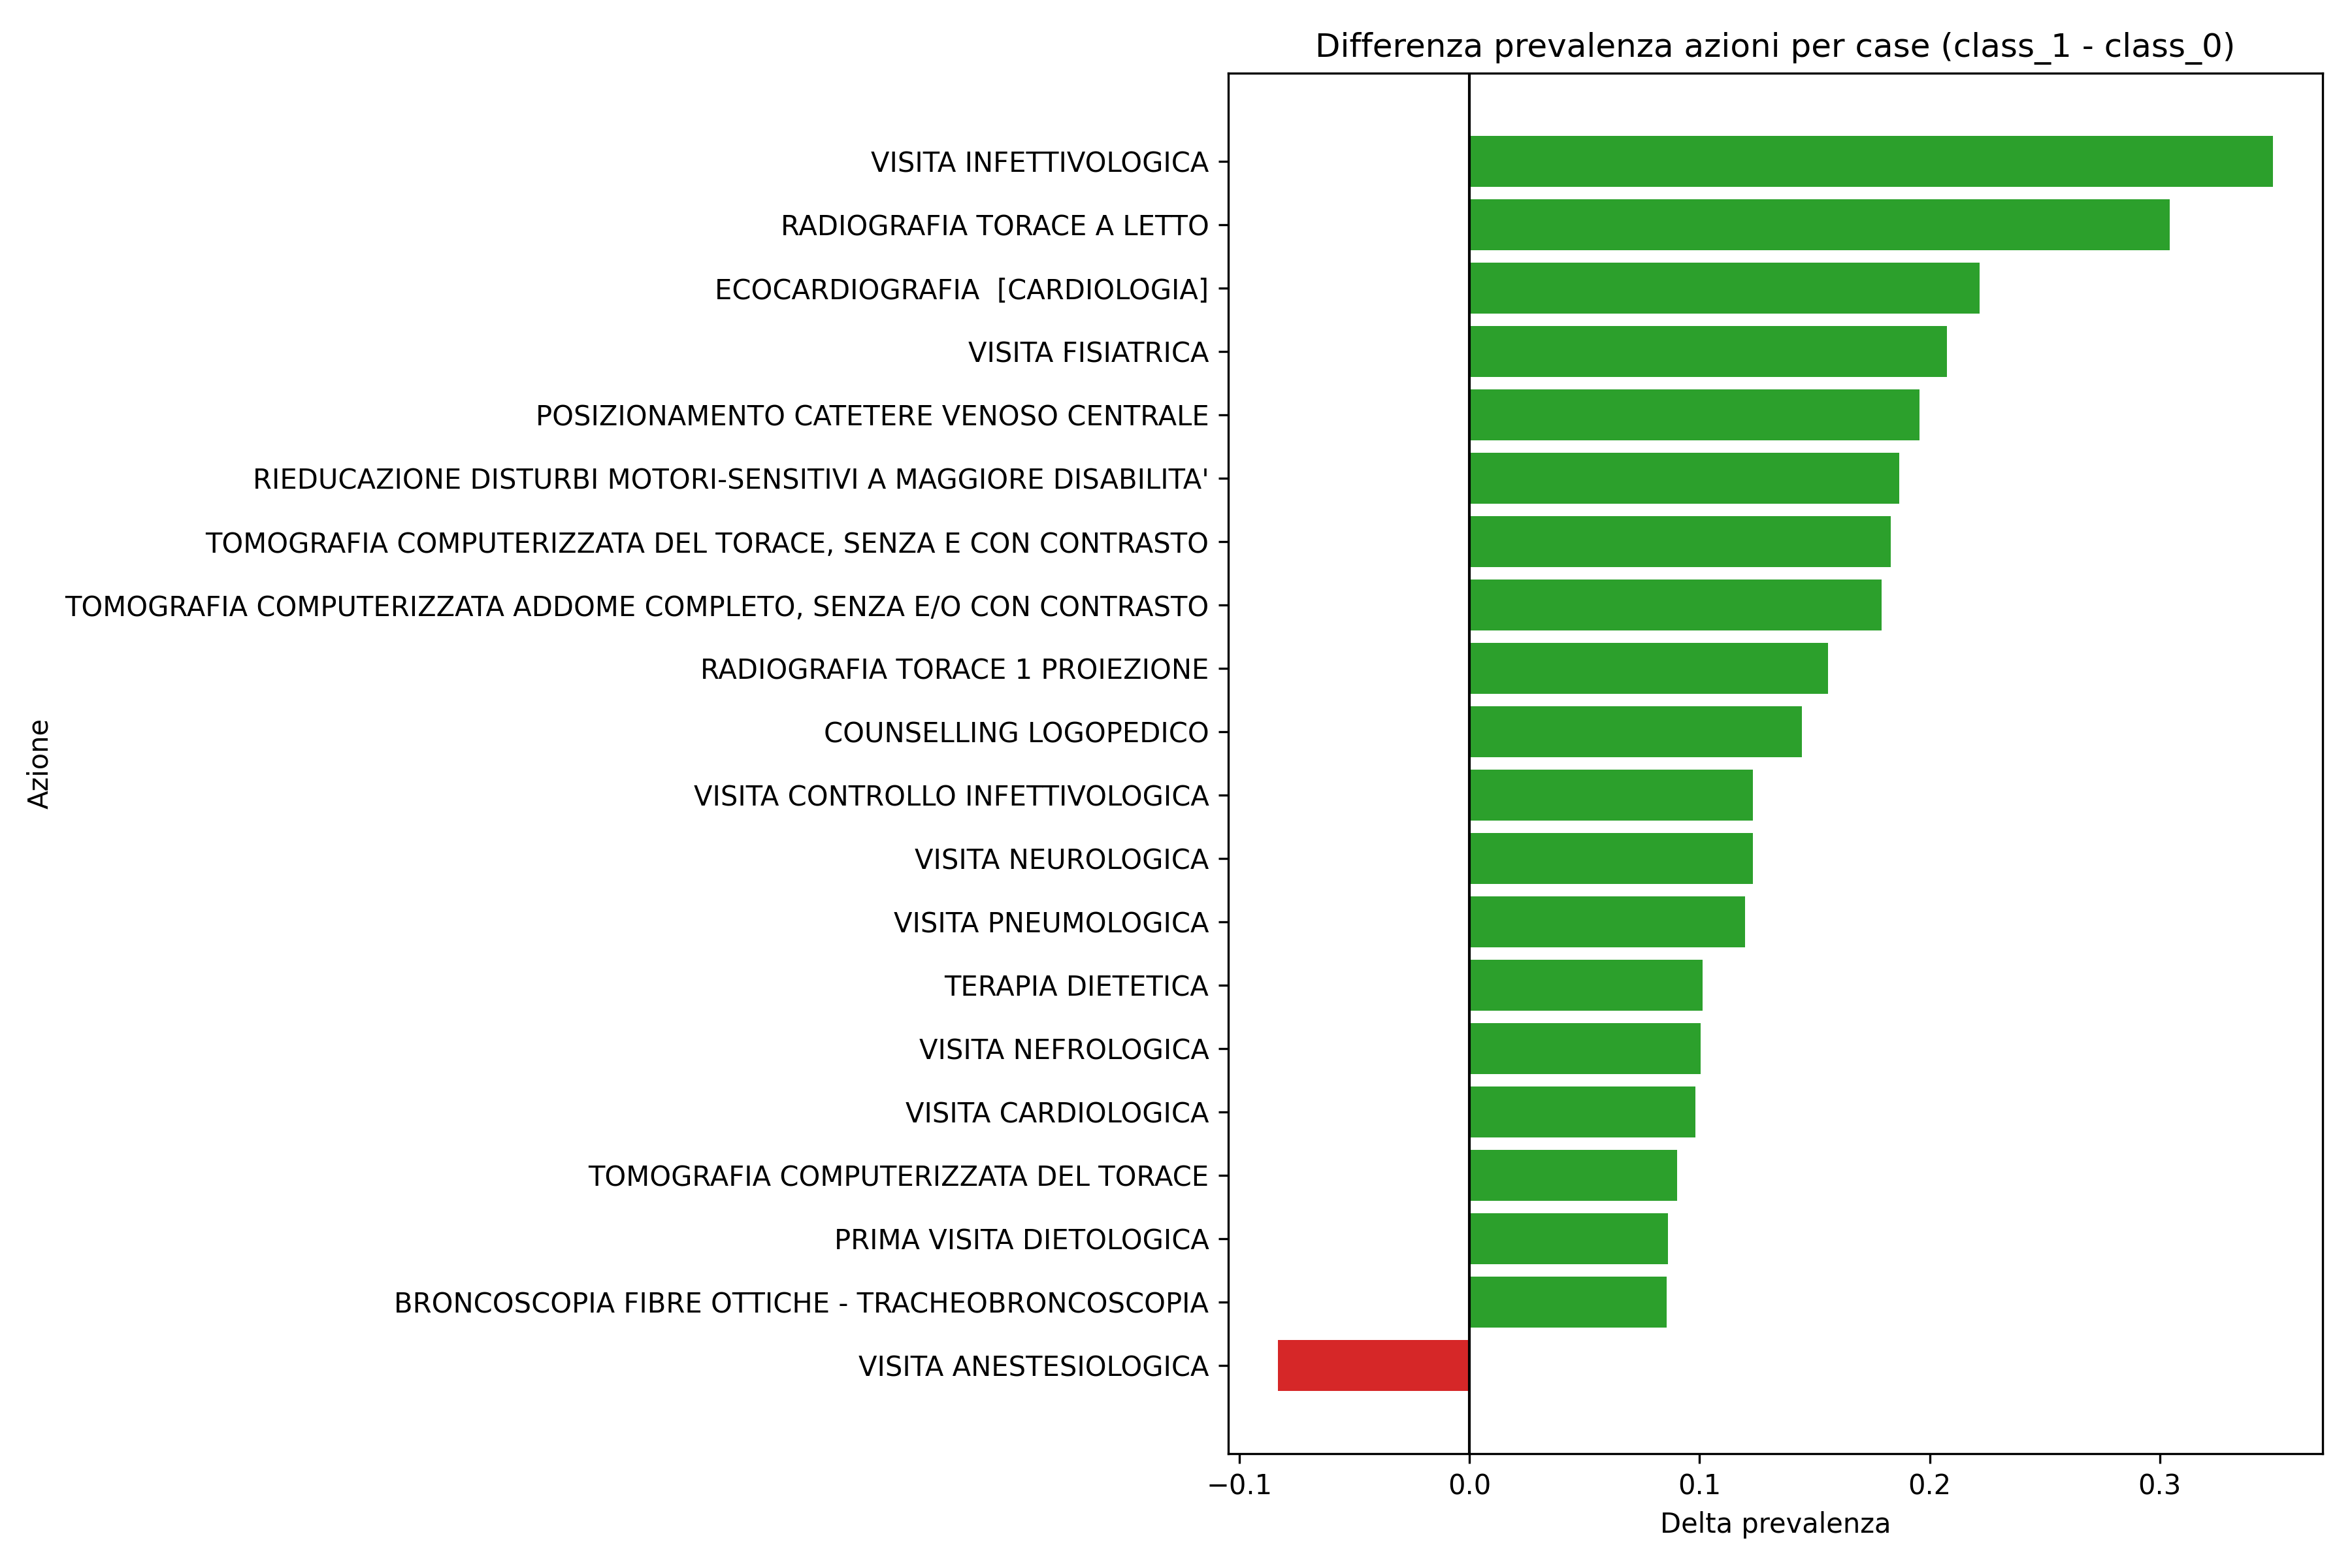
\includegraphics[width=\linewidth]{class_action_prevalence_diff_top.png}
      {\small\itshape Delta di prevalenza per azione:\\
      alcune procedure correlano fortemente\\con LOS critico.}
    \end{column}
  \end{columns}
\end{frame}

% ── SLIDE 6: BERT + Focal Loss ────────────────────────────────
\begin{frame}{Il Modello: BERT e la Focal Loss}
  \begin{columns}[T]
    \begin{column}{0.50\textwidth}
      \textbf{Architettura:} \texttt{bert-base-uncased} + classification head
      \begin{itemize}
        \item 110M parametri, tokenizer WordPiece
        \item Perché non ClinicalBERT? \alert{Vocabulary mismatch}:\\
              nomenclature locali non standardizzate
        \item Fine-tuning con Stratified 5-Fold CV
      \end{itemize}

      \vspace{0.4em}
      \begin{block}{Focal Loss — Formula}
        \[
          FL(p_t) = -\alpha_t\,(1-p_t)^{\gamma}\,\log(p_t)
        \]
        Il fattore $(1-p_t)^\gamma$ \textbf{abbatte il gradiente}
        degli esempi facili (classe 0 dominante), forzando BERT
        ad imparare i casi rari di long-LOS.
      \end{block}
    \end{column}

    \begin{column}{0.47\textwidth}
      \centering
      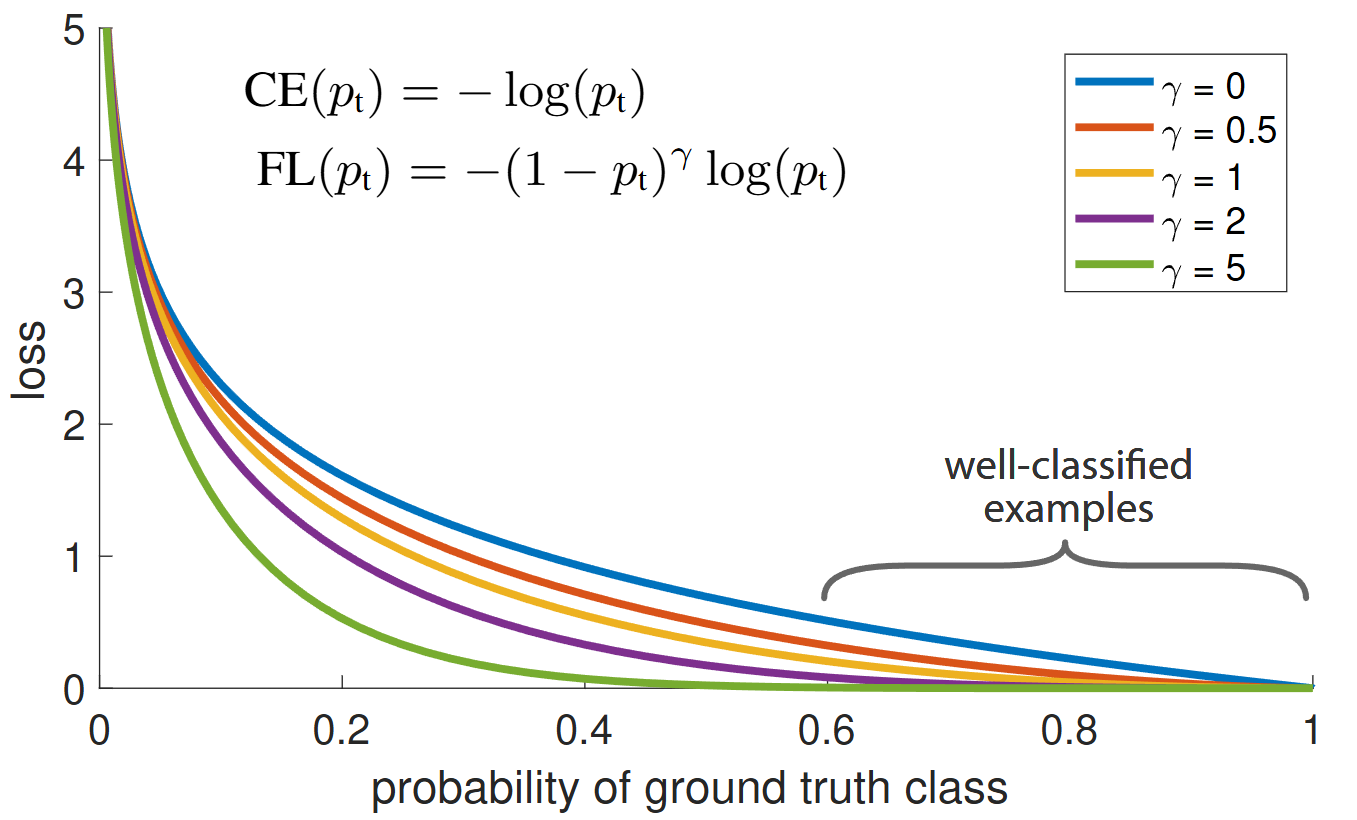
\includegraphics[width=\linewidth]{focal loss fig 1.png}
      {\small\itshape Al crescere di $\gamma$, la loss sugli esempi\\
      facili ($p_t \to 1$) crolla: il modello si \alert{concentra}\\
      sui casi complessi e rari.}
    \end{column}
  \end{columns}
\end{frame}

% ── SLIDE 7: Risultati Classificazione ───────────────────────
\begin{frame}{Risultati: Balanced Accuracy 88\%}
  \begin{columns}[T]
    \begin{column}{0.55\textwidth}
      \begin{block}{Confronto Embedding — Metriche Chiave}
        \footnotesize
        \renewcommand{\arraystretch}{1.3}
        \begin{tabular}{lccc}
          \toprule
          \textbf{Embedding} & \textbf{Bal.\ Acc.} & \textbf{Recall} & \textbf{Prec.} \\
          \midrule
          Array Concat. & 83.44\% & 78.51\% & 45.24\% \\
          Binning       & 87.16\% & 81.82\% & 57.23\% \\
          \alert{\textbf{Storytelling}} & \alert{\textbf{89.69\%}} & \alert{\textbf{85.95\%}} & \alert{\textbf{61.54\%}} \\
          \bottomrule
        \end{tabular}
      \end{block}

      \vspace{0.5em}
      \textbf{Matrice di confusione — Storytelling:}
      \footnotesize
      \renewcommand{\arraystretch}{1.3}
      \begin{tabular}{cc|c|c|}
        & & \multicolumn{2}{c|}{\textbf{Predetto}} \\
        & & Normale & Critico \\
        \cline{3-4}
        \multirow{2}{*}{\textbf{Reale}} & Normale & 923 & 65 \\
        \cline{3-4}
        & Critico & \alert{17} & \textbf{104} \\
        \cline{3-4}
      \end{tabular}
    \end{column}

    \begin{column}{0.42\textwidth}
      \begin{alertblock}{Il Trade-off Clinico}
        \textbf{Recall 85.95\%} = pochi falsi negativi.

        In ambito medico, \alert{non identificare} un paziente
        critico è un danno grave: percorso inatteso, letti
        occupati a sorpresa, dimissioni abortite.

        \vspace{0.3em}
        Falsi positivi (Precision 61.54\%) = allerta
        preventiva: il costo è tollerabile e gestibile.
      \end{alertblock}

      \vspace{0.3em}
      {\footnotesize\itshape La Focal Loss è la chiave:\\
      solo 17 falsi negativi su 121 casi critici.}
    \end{column}
  \end{columns}
\end{frame}

% ── SLIDE 8: XAI — Black Box ──────────────────────────────────
\section{Explainable AI}

\begin{frame}{Il Problema della Black-Box in Sanità}
  \begin{columns}[T]
    \begin{column}{0.55\textwidth}
      Il modello \textbf{funziona} — ma il medico deve \textbf{fidarsi}.

      \vspace{0.5em}
      \begin{alertblock}{Il Paradosso della Black-Box}
        Una rete neurale è un oracolo opaco: restituisce
        una probabilità, ma \alert{non spiega perché}.\\
        In sanità questo è inaccettabile per il clinico.
      \end{alertblock}

      \vspace{0.5em}
      \textbf{Già disponibili in letteratura:}
      \begin{itemize}
        \item Grad-CAM $\to$ progettato per CNN/immagini
        \item Vanilla Gradient $\to$ soggetto a \textit{gradient shattering}
        \item SmoothGrad / Blur IG $\to$ incompatibili con embedding discreti
      \end{itemize}

      \vspace{0.3em}
      \textbf{Soluzione adottata:} \alert{Integrated Gradients (IG)}\\
      — assiomaticamente verificabili, corretti per sequenze testuali.
    \end{column}

    \begin{column}{0.42\textwidth}
      \centering
      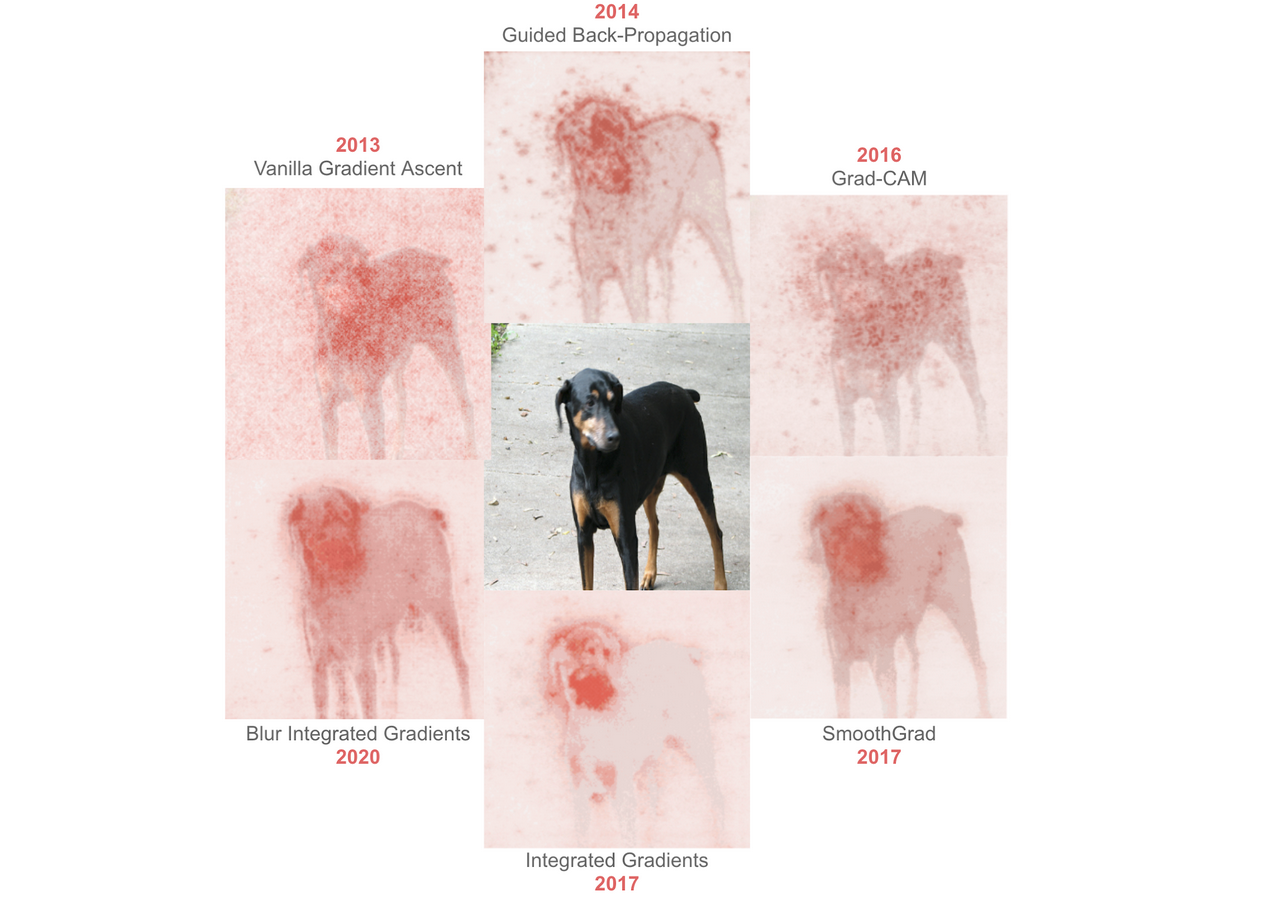
\includegraphics[width=\linewidth]{comparison_with_a_dog.png}
      {\small\itshape I metodi classici producono maschere\\
      ad alto rumore. IG fornisce attribuzioni\\
      stabili e semanticamente coerenti.}
    \end{column}
  \end{columns}
\end{frame}

% ── SLIDE 9: Integrated Gradients ────────────────────────────
\begin{frame}{Integrated Gradients e la Baseline \texttt{[PAD]}}
  \begin{columns}[T]
    \begin{column}{0.55\textwidth}
      \textbf{Intuizione:} misurare il contributo di ogni token
      integrando i gradienti lungo un percorso dalla
      \alert{baseline} (assenza d'informazione) all'input reale.

      \vspace{0.4em}
      \begin{block}{Formula Adattiva (Riemann Trapezoid)}
        \footnotesize
        \[
          IG_i^{\approx}(x) \coloneqq (x_i - x'_i) \times
          \frac{1}{m}\sum_{k=1}^{m}
          \frac{\partial F\!\left(x' + \tfrac{k}{m}(x-x')\right)}{\partial x_i}
        \]
      \end{block}

      \begin{block}{La Baseline}
        $x' = $ vettore di token \texttt{[PAD]} (ID=0):
        \alert{zero semantico} per i BERT embedding.\\
        Garantisce l'Assioma di Sensibilità.
      \end{block}

      \vspace{0.3em}
      {\footnotesize
      \textbf{Convergenza adattiva:}
      90\% dei campioni converge a $m{=}1500$ steps;\\
      picchi fino a $m{=}5500$ per tracce molto lunghe.}
    \end{column}

    \begin{column}{0.42\textwidth}
      \begin{alertblock}{Completeness — Verifica}
        \footnotesize
        \[
          \text{Rel\_Error} = \frac{|f(x) - f(x') - \sum \text{Attr}|}{|f(x)-f(x')|}
        \]
        Accettabile se $\le 5\%$.\\
        Garantisce che le attribuzioni spieghino\\
        \textit{tutta} la differenza di output.
      \end{alertblock}

      \vspace{0.5em}
      \begin{exampleblock}{Ottimizzazione Hardware}
        \footnotesize
        Riemann Trapezoid vs Gauss-Legendre:\\
        da \alert{15~s/campione} a \textbf{2.5~s/campione}\\
        scaricando il calcolo sulla GPU RTX 4090.
      \end{exampleblock}
    \end{column}
  \end{columns}
\end{frame}

% ── SLIDE 10: Aggregazione Sub-Token ─────────────────────────
\begin{frame}{La Sfida: Aggregazione dei Sub-Token}
  \textbf{WordPiece frammenta} le parole cliniche in sub-token privi
  di significato autonomo. \alert{Serve ricostruirle.}

  \vspace{0.5em}
  \begin{columns}[T]
    \begin{column}{0.52\textwidth}
      \textbf{Step A — da 768 dimensioni a scalar:}\\
      $\text{sum}(\text{dim}=-1)$ collassa il vettore IG in un
      singolo valore per token.

      \vspace{0.4em}
      \textbf{Step B — root sum dei \texttt{\#\#} fragments:}\\
      I sub-token marcati \texttt{\#\#} sommano il loro score
      al token radice $\to$ parola clinica intera.

      \vspace{0.4em}
      Token artificiali \texttt{[CLS]}, \texttt{[SEP]} esclusi.

      \vspace{0.4em}
      \begin{exampleblock}{Risultato}
        Ogni \textbf{azione clinica reale} ottiene un
        unico score aggregato, leggibile dal clinico.
      \end{exampleblock}
    \end{column}

    \begin{column}{0.45\textwidth}
      \centering
      % scalebox: il diagramma tikz è ~6.8cm, la colonna ~5.7cm in 16:9
      \scalebox{0.78}{%
      \begin{tikzpicture}[
        node distance=1.5cm,
        box/.style={rectangle, draw=primary!80, fill=primary!8!lightbg,
          thick, minimum height=0.7cm, minimum width=2.0cm,
          rounded corners=2pt, align=center, font=\small},
        finalbox/.style={rectangle, draw=successgreen!70!black,
          fill=successgreen!10, thick, minimum height=0.8cm,
          minimum width=2.6cm, rounded corners=2pt, align=center,
          font=\small\bfseries},
        arr/.style={-Stealth, thick, color=darktext!60},
        lbl/.style={font=\tiny\bfseries, color=alertred},
      ]
        \node[box] (card) {\texttt{card}};
        \node[box, right=0.4cm of card] (iolo) {\texttt{\#\#iology}};
        \node[box, right=0.4cm of iolo] (vis)  {\texttt{visit}};

        \node[lbl, below=0.1cm of card]  {IG: $+12.45$};
        \node[lbl, below=0.1cm of iolo]  {IG: $+7.83$};
        \node[lbl, below=0.1cm of vis]   {IG: $+18.92$};

        \node[finalbox, below=1.2cm of card, xshift=1.2cm]
          (fcardio) {\textbf{Cardiology}};
        \node[font=\tiny\bfseries\color{successgreen!70!black},
          below=0.1cm of fcardio] {score: $+20.28$};

        \node[finalbox, below=1.2cm of vis]
          (fvis) {\textbf{visit}};
        \node[font=\tiny\bfseries\color{successgreen!70!black},
          below=0.1cm of fvis] {score: $+18.92$};

        \draw[arr] (card.south) -- (fcardio.north west);
        \draw[arr] (iolo.south) -- (fcardio.north east);
        \draw[arr] (vis.south)  -- (fvis.north);
      \end{tikzpicture}}
      \vspace{0.2em}
      {\small\itshape Ricomposizione ``Cardiology visit''.}
    \end{column}
  \end{columns}
\end{frame}

% ── SLIDE 11: Cruscotto Clinico ★ ────────────────────────────
\begin{frame}{Il Cruscotto Clinico: Reparto 701 Cardiochirurgia}
  \textbf{109 pazienti — Ospedale di Alessandria.}
  BERT + IG identificano i \alert{colli di bottiglia processuali}.

  \vspace{0.3em}
  \begin{columns}[T]
    \begin{column}{0.48\textwidth}
      \centering
      \includegraphics[width=\linewidth]%
        {histogram_actions_narrativo_bert-base-uncased_single_20260226_195041.png}
      {\small\itshape Top Actions: punteggi IG aggregati\\
      per azione clinica (scala logaritmica).}
    \end{column}
    \begin{column}{0.49\textwidth}
      \centering
      \includegraphics[width=\linewidth]%
        {heatmap_actions_narrativo_bert-base-uncased_single_20260226_195041.png}
      {\small\itshape Heatmap intra-traccia: l'intensità cromatica\\
      isola il collo di bottiglia nella sequenza.}
    \end{column}
  \end{columns}
\end{frame}

% ── SLIDE 12: Fattibilità Aziendale ─────────────────────────
\section{Conclusioni}

\begin{frame}{Fattibilità Aziendale e Costi di Deployment}
  \begin{columns}[T]
    \begin{column}{0.52\textwidth}
      \textbf{Hardware:} RTX 4090 | AMD Ryzen 9 5900X | 64 GB RAM

      \vspace{0.5em}
      \begin{block}{Metriche Wall-Clock (1.109 pazienti)}
        \renewcommand{\arraystretch}{1.2}
        \begin{tabular}{lr}
          \toprule
          \textbf{Fase} & \textbf{Tempo} \\
          \midrule
          Parsing XES $\to$ Storytelling & 1~min \\
          Fine-tuning BERT (5 epoche) & 6~min~30~s \\
          Estrazione IG (109 tracce) & 8~min~16~s \\
          \midrule
          \textbf{Overhead totale (1.109 paz.)} & \alert{\textbf{$\approx$ 80 min}} \\
          \bottomrule
        \end{tabular}
      \end{block}
    \end{column}

    \begin{column}{0.44\textwidth}
      \begin{exampleblock}{Scenario Reale}
        \textbf{Trigger notturno automatico:}
        \begin{enumerate}
          \item Esportazione asincrona dal DB ospedaliero
          \item Pipeline IG in background
          \item \textbf{Report pronto al mattino} per il case manager
        \end{enumerate}
      \end{exampleblock}

      \vspace{0.4em}
      Il sistema è \textbf{reale e sostenibile}:\\
      nessun hardware live aggiuntivo,\\
      nessun cloud dedicato obbligatorio.
    \end{column}
  \end{columns}
\end{frame}

% ── SLIDE 13: Conclusioni ─────────────────────────────────────
\begin{frame}{Conclusioni e Sviluppi Futuri}
  \begin{columns}[T]
    \begin{column}{0.50\textwidth}
      \textbf{Risultati raggiunti:}
      \begin{itemize}
        \item Pipeline end-to-end: XES $\to$ Storytelling $\to$ BERT $\to$ IG
        \item Balanced Accuracy \textbf{89.69\%} con sbilanciamento 89/11
        \item Cruscotto clinico leggibile per le amministrazioni
        \item Fattibilità computazionale \textbf{dimostrata empiricamente}
      \end{itemize}

      \vspace{0.5em}
      \begin{alertblock}{Limite Fondamentale}
        IG e Attention Maps misurano \textbf{correlazione},
        non causalità. La valutazione clinica finale
        spetta sempre allo \alert{specialista umano}.
      \end{alertblock}
    \end{column}

    \begin{column}{0.47\textwidth}
      \begin{block}{Sviluppi Futuri — TEXLOS}
        Da analisi \textit{post-mortem} a classificazione
        \textbf{runtime}:
        \begin{itemize}
          \item \textit{Next-Activity-Prediction} con IG parziali
          \item XAI ad alta densità ai checkpoint quotidiani
          \item Logiche manageriali \textbf{proattive} in tempo reale
        \end{itemize}
      \end{block}

      \vspace{0.5em}
      \centering
      \Large\textbf{Grazie per l'attenzione.}\\
      \normalsize\vspace{0.3em}
      \textit{Domande?}
    \end{column}
  \end{columns}
\end{frame}

% ============================================================
%  BACKUP SLIDES  (non contano nel timer)
% ============================================================
\appendix

% ── SLIDE 14 (B): Hardware & Hyperparameter Tuning ───────────
\begin{frame}{(Backup) Hardware e Hyperparameter Tuning}
  \begin{columns}[T]
    \begin{column}{0.50\textwidth}
      \textbf{Setup Sperimentale:}
      \begin{itemize}
        \item GPU: \textbf{NVIDIA GeForce RTX 4090}
        \item CPU: AMD Ryzen 9 5900X (12 core / 24 thread)
        \item RAM: 64 GB
      \end{itemize}

      \vspace{0.4em}
      \textbf{Perché non BERT-Large?}
      \begin{itemize}
        \item Batch size: da 22 (base) a \alert{4} (large) per VRAM
        \item 5-Fold CV materialmente impraticabile
        \item \textit{Data plateauing}: 7.000 tracce non saturano 340M params
      \end{itemize}
    \end{column}

    \begin{column}{0.47\textwidth}
      \begin{block}{Ottimizzazione con Optuna}
        Esplorazione bayesiana automatica degli iperparametri:
        \begin{itemize}
          \item Learning rate, batch size, dropout
          \item Parametri Focal Loss ($\alpha$, $\gamma$)
          \item Early stopping: patience = 5, $\Delta_{\min} = 10^{-3}$
        \end{itemize}
        Miglior checkpoint: \textbf{epoca 10} su 15 totali.
      \end{block}

      \vspace{0.3em}
      \centering
      \includegraphics[width=0.9\linewidth]{train_val_loss.png}
      {\small\itshape Curva Training vs Validation Loss.}
    \end{column}
  \end{columns}
\end{frame}

% ── SLIDE 15 (B): Esperimento LLM fallito ────────────────────
\begin{frame}{(Backup) L'Esperimento Fallito: Data Augmentation con LLM}
  \begin{columns}[T]
    \begin{column}{0.48\textwidth}
      \textbf{Obiettivo:} sintetizzare nuove tracce per la classe
      minoritaria usando LLM generativi locali (Ollama).

      \vspace{0.3em}
      Modelli testati: \texttt{phi4:14b}, \texttt{nous-hermes2:34b}\\
      Temperature fissata a $T = 0.0$ per ridurre le allucinazioni.

      \vspace{0.3em}
      \begin{alertblock}{Problema: Allucinazioni Semantiche}
        I modelli aggiungono \textbf{descrizioni procedurali inventate}
        (\textit{``to evaluate intracranial hemorrhages\ldots''}) o
        dettagli non nel DB (\textit{``with contrast medium''}).

        Il rumore lessicale \alert{distorce l'attenzione} di BERT
        sui delta temporali, degradando i risultati.
      \end{alertblock}
    \end{column}

    \begin{column}{0.49\textwidth}
      \begin{block}{Esempio — Output di \texttt{phi4:14b}}
        {\tiny
        \textit{``\ldots The Complete abdomen ultrasound was performed as the
        initial examination to assess abdominal structures for any
        abnormalities or pathologies that might require further
        investigation. This non-invasive imaging technique provided
        valuable insights into the patient's abdominal condition\ldots''}}
      \end{block}

      \vspace{0.3em}
      \begin{exampleblock}{Lezione Appresa}
        La pipeline richiede dati \textbf{originali e fedeli} al
        nomenclatore locale. Lo storytelling sintetico introduce
        vocabolario estraneo che compromette la
        confrontabilità con le tracce reali.
      \end{exampleblock}
    \end{column}
  \end{columns}
\end{frame}

% ============================================================
\end{document}
